\documentclass[journal,12pt,onecolumn]{IEEEtran}
\usepackage{cite}
\usepackage{graphicx}
\usepackage{amsmath,amssymb,amsfonts,amsthm}
\usepackage{algorithmic}
\usepackage{textcomp}
\usepackage{xcolor}
\usepackage{txfonts}
\usepackage{listings}
\usepackage{enumitem}
\usepackage{mathtools}
\usepackage{gensymb}
\usepackage{comment}
\usepackage[breaklinks=true]{hyperref}
\usepackage{tkz-euclide} 
\usepackage{caption}
\usepackage{listings}
\usepackage{gvv}                                        
\usepackage[latin1]{inputenc} 

\usetikzlibrary{arrows.meta, positioning}
\usepackage{xparse}
\usepackage{color}                                            
\usepackage{array}                                            
\usepackage{longtable}                                       
\usepackage{calc}                                             
\usepackage{multirow}
\usepackage{multicol}
\usepackage{hhline}                                           
\usepackage{ifthen}                                           
\usepackage{lscape}
\usepackage{tabularx}
\usepackage{array}
\usepackage{float}
\newtheorem{theorem}{Theorem}[section]
\newtheorem{problem}{Problem}
\newtheorem{proposition}{Proposition}[section]
\newtheorem{lemma}{Lemma}[section]
\newtheorem{corollary}[theorem]{Corollary}
\newtheorem{example}{Example}[section]
\newtheorem{definition}[problem]{Definition}
\newcommand{\BEQA}{\begin{eqnarray}}
\newcommand{\EEQA}{\end{eqnarray}}
\usepackage{float}
\theoremstyle{remark}
\usepackage{circuitikz}
\usepackage{tikz}\title{}
\title{\Huge MN:MINING ENGINEERING}
\author{Vaishnavi Ramkrishna Anantheertha-EE25BTECH11059}
\begin{document}
\maketitle

\section*{Q.1--Q.5 carry one mark each}
\begin{enumerate}
\item Choose the most appropriate word from the options given below to complete the following sentence.
\vspace{0.5em}

A person suffering from Alzheimer disease \underline{\hspace{3cm}} short-term memory loss.

\vspace{0.5em}
\hfill\brak{GATE\ MN\ 2014}
\begin{multicols}{4}
\begin{enumerate}
\item experienced
\item has experienced
\item is experiencing
\item experiences
\end{enumerate}
\end{multicols}
\item Choose the most appropriate word from the options given below to complete the following
sentence
\vspace{0.5em}

\underline{\hspace{3cm}} he key to their happiness; they are satisfied with what they have 

\vspace{0.5em}
\hfill\brak{GATE\ MN\ 2014}
\begin{multicols}{4}
\begin{enumerate}
\item Contentment 
\item Ambition 
\item Perseverance 
\item Hunger
\end{enumerate}
\end{multicols}
\item Which of the following options is the closest in meaning to the sentence below?
\vspace{0.5em}
\textbf{As a woman, I have no country.}

\hfill\brak{GATE\ MN\ 2014}    
\begin{enumerate}
    \item Women have no country.
    \item Women are not citizens of any country.
    \item Womens solidarity knows no national boundaries
    \item Women of all countries have equal legal rights
\end{enumerate}
\item In any given year, the probability of an earthquake greater than Magnitude 6 occurring in the
Garhwal Himalayas is 0.04. The average time between successive occurrences of such earthquakes
is  \underline{\hspace{3cm}} years.

\hfill\brak{GATE\ MN\ 2014}

\item The population of a new city is 5 million and is growing at 20\% annually. How many years would
it take to double at this growth rate?

\hfill\brak{GATE\ MN\ 2014} 
\begin{multicols}{4}
\begin{enumerate}
\item $3$-$4$ years
\item $4$-$5$ years
\item $5$-$6$ years
\item $6$-$7$ years
\end{enumerate}
\end{multicols}
\section*{Q6 to Q10 carries 2 marks}
\item In a group of four children, Som is younger to Riaz. Shiv is elder to Ansu. Ansu is youngest in the group. Which of the following statements is/are required to find the eldest child in the group?

\textbf{Statements}
\hfill\brak{GATE\ MN\ 2014}
\begin{enumerate}[label=\arabic*]
\item Shiv is younger to Riaz.
\item Shiv is elder to Som.
\end{enumerate}

\begin{enumerate}
    \item Statement 1 by itself determines the eldest child.
    \item Statement 2 by itself determines the eldest child.
    \item Statements 1 and 2 are both required to determine the eldest child.
    \item Statements 1 and 2 are not sufficient to determine the eldest child.
\end{enumerate}

\item Moving into a world of big data will require us to change our thinking about the merits of
exactitude. To apply the conventional mindset of measurement to the digital, connected world of
the twenty-first century is to miss a crucial point. As mentioned earlier, the obsession with
exactness is an artefact of the information-deprived analog era. When data was sparse, every data
point was critical, and thus great care was taken to avoid letting any point bias the analysis.
From BIG DATA Viktor Mayer-Schonberger and Kenneth Cukier
The main point of the paragraph is $\colon$

\hfill\brak{GATE\ MN\ 2014}
\begin{enumerate}
\item The twenty-first century is a digital world
\item Big data is obsessed with exactness 
\item Exactitude is not critical in dealing with big data
\item Sparse data leads to a bias in the analysis
\end{enumerate}

\item The total exports and revenues from the exports of a country are given in the two pie charts below. The pie chart for exports shows the quantity of each item as a percentage of the total quantity of exports. The pie chart for the revenues shows the percentage of the total revenue generated through export of each item. The total quantity of exports of all the items is 5 lakh tonnes and the total revenues are 250 crore rupees. What is the ratio of the revenue generated through export of Item 1 per kilogram to the revenue generated through export of Item 4 per kilogram?
\begin{figure}[H]
  \centering
  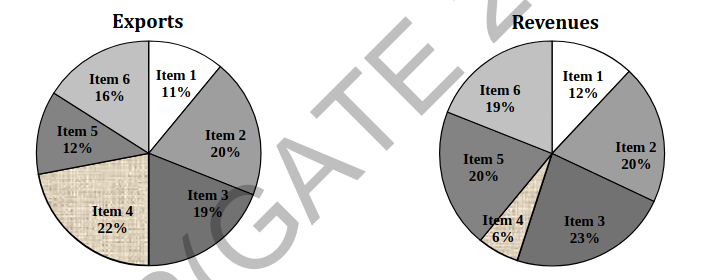
\includegraphics[width=0.4\columnwidth]{figs/graph1.png}
  \caption{EXPORT AND REVENUES}
  \label{fig:ladder}
\end{figure}

\hfill\brak{GATE\ MN\ 2014}
\begin{multicols}{4}
\begin{enumerate}
\item $1$$\colon$$2$
\item $2$$\colon$$1$
\item $1$$\colon$$4$
\item $4$$\colon$$1$
\end{enumerate}
\end{multicols}
\item X is 1 km northeast of Y. Y is $1$ km southeast of Z. W is $1$ km west of Z. P is $1$ km south of W. Q is $1$ km east of P. What is the distance between X and Q in km?

\hfill\brak{GATE\ MN\ 2014}
  \begin{multicols}{4}
  \begin{enumerate}
    \item $1$
    \item $\sqrt{2}$
    \item $\sqrt{3}$
    \item $2$
\end{enumerate}
 \end{multicols}
\item 10\% of the population in a town is $HIV$. A new diagnostic kit for HIV detection is available; this kit correctly identifies HIV$^+$ individuals $95$\% of the time, and HIV$^-$ individuals 89\% of the time. A particular patient is tested using this kit and is found to be positive. The probability that the individual is actually positive is \underline{\hspace{2cm}}.
\end{enumerate}

\hfill\brak{GATE\ MN\ 2014}
\section*{Q. 1 to Q. 25 carry one mark each.}
\begin{enumerate}
\item A block of weight 100 kN rests on a floor as shown in the figure. The coefficient of static friction between the block and the floor is $0.5$. A force of 45 kN is applied horizontally on the block. The static frictional force in kN is
\begin{figure}[H]
  \centering
  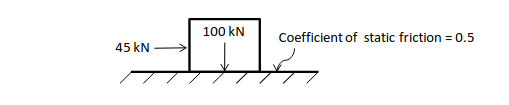
\includegraphics[width=0.4\columnwidth]{figs/spring block.png}
  \caption{spring block system}
  \label{fig:block}
\end{figure}


\hfill\brak{GATE\ MN\ 2014}
\begin{multicols}{4}
\begin{enumerate}
\item $22.5$
\item $50.0$
\item $55.0 $
\item $100.0$
\end{enumerate}
\end{multicols}
\item A spring of constant stiffness k is stretched from point A to point B (displacement u in the figure) by a force F. The potential energy of the spring is expressed by
\begin{figure}[H]
  \centering
  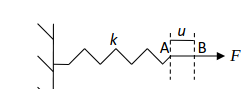
\includegraphics[width=0.4\columnwidth]{figs/spring2.png}
  \caption{spring block system}
  \label{fig:spring}
\end{figure}

\hfill\brak{GATE\ MN\ 2014}
\begin{multicols}{2}
\begin{enumerate}
\item $\frac{1}{2}ku^2 - Fu$
\item $\frac{1}{2}ku^2 + Fu$
\item $ku-F$
\item $ku+F$
\end{enumerate}
\end{multicols}
\item If $\sigma_s$ is the induced stress and $\sigma_i$ is the in-situ stress at a point below ground, the stress concentration at that point is

\hfill\brak{GATE\ MN\ 2014}
\begin{multicols}{2}
\begin{enumerate}
  \item $\sqrt{\dfrac{\sigma_s}{\sigma_i}}$
  \item $\sqrt{\dfrac{\sigma_i}{\sigma_s}}$
  \item $\dfrac{\sigma_i}{\sigma_s}$
  \item $\dfrac{\sigma_s}{\sigma_i}$
\end{enumerate}
\end{multicols}

 \item The components of state of stress at a point in $x$--$y$ plane are given as 
$\sigma_{xx} = 5\,\text{MPa}$, $\sigma_{yy} = 10\,\text{MPa}$ and 
$\tau_{xy} = -2\,\text{MPa}$. The sum of the principal stresses acting on the 
$x$--$y$ plane in MPa is \underline{\hspace{2cm}}.

\hfill\brak{GATE\ MN\ 2014}

\item The angle $5^\circ 15' 25''$ is expressed in hours, minutes, and seconds as

\hfill\brak{GATE\ MN\ 2014}
\begin{multicols}{2}
\begin{enumerate}
\item $1^h 20^{min} 1.67^s$
\item  $1^h 20^{min} 16.00^s$ 
\item $0^h 21^{min} 1.67^s$
\item $0^h 21^{min} 16.00^s$
\end{enumerate}
\end{multicols}

\item A circular curve has a radius of 200 m and deflection angle of $65^\circ$.the length of the curve in m is

\hfill\brak{GATE\ MN\ 2014}
\begin{multicols}{4}
\begin{enumerate}
\item $221$
\item $227$
\item $235$
\item $262$
\end{enumerate}
\end{multicols}
\item The weight strength of ANFO of specific gravity $0.8$ is $912~\text{kcal/kg}$. The weight strength of an emulsion explosive of specific gravity $1.2$ is $850~\text{kcal/kg}$. Bulk strength of the emulsion explosive relative to ANFO in percentage is \underline{\hspace{2cm}}.
\hfill\brak{GATE\ MN\ 2014}
\item In a cut-and-fill stope, the main purpose of back filling is to
\begin{multicols}{2}
\begin{enumerate}
\item reduce ore dilution  
\item prevent high stress concentrations in far field domain  
\item prevent displacement due to dilation of fractured wall rock  
\item improve ore rehandling 
\end{enumerate}
\end{multicols}

\item Bypass valve in a compressed oxygen type self-contained breathing apparatus is meant to
\hfill\brak{GATE\ MN\ 2014}

\begin{enumerate}
\item release accumulated nitrogen in the breathing bag
\item release excess pressure in the breathing bag
\item supply oxygen directly to wearer in case pressure reducing valve 
\item flush out the apparatus with oxygen on opening the cylinder valve 
\end{enumerate}
\item Given S is the setting load and Y is the yield load of a hydraulic prop, the correct relationship is

\hfill\brak{GATE\ MN\ 2014}

\begin{multicols}{4}
\begin{enumerate}
\item $S \leq Y$ 
\item $S \geq Y$
\item $S = Y$
\item $S = Y^{2}$
\end{enumerate}
\end{multicols}
\item Solution of the differential equation $\frac{dy}{dx} = ky$ follows exponential decay (where $k$ is a constant) for x $\in [0, \infty)$ if

\hfill\brak{GATE\ MN\ 2014}
\begin{multicols}{4}
\begin{enumerate}
\item $k \geq 0$ 
\item $k \leq 0$ 
\item $k=0$
\item $k=e$
\end{enumerate}
\end{multicols}
\item The value of $k$ for which the vectors $\mathbf{a} = 2\mathbf{i} - 3\mathbf{j}$ and $\mathbf{b} = k \mathbf{i} + 4 \mathbf{j}$ are orthogonal to each other is \underline{\hspace{2cm}}.

\item Which one of the following is the most likely mode of slope failure for waste dump

\hfill\brak{GATE\ MN\ 2014}

\begin{multicols}{2}
\begin{enumerate}
\item Circular 
\item Wedge  
\item Plane
\item Toppling
  
\end{enumerate}
\end{multicols}
\item \quad The occurrence of head in a single toss of an unbiased coin is given by a random variable $X$. The variance of $X$ is \underline{\hspace{3cm}}.

\hfill\brak{GATE\ MN\ 2014}

\item The divergence of the vector $\mathbf{v} = (x+y)(-y \mathbf{i} + x \mathbf{j})$ is

\hfill\brak{GATE\ MN\ 2014}
\begin{multicols}{4}
\begin{enumerate}
\item $y - x$
\item $x - y$
\item $x^2 - y^2$
\item $y^2 - x^2$
\end{enumerate}
\end{multicols}


\item The $\displaystyle \lim_{x \to 0} \frac{|x|}{x}$ is

\hfill\brak{GATE\ MN\ 2014}
\begin{multicols}{4}
\begin{enumerate}
\item $-1$
\item $0$
\item $1$
\item non-existent
\end{enumerate}
\end{multicols}
\item For Indian coal mines, the maximum allowable concentration of respirable dust containing 7.5\% free silica in $mg/m^3$ is

\hfill\brak{GATE\ MN\ 2014}
\begin{multicols}{4}
\begin{enumerate}
\item $2.0$
\item $2.2$
\item $2.5$
\item $2.7$
\end{enumerate}
\end{multicols}
\item  Given $k$ is the thermal conductivity, $\rho$ is density and $c$ is specific heat of a rock sample, the thermal diffusivity of the rock sample is

\hfill\brak{GATE\ MN\ 2014}
\begin{multicols}{4}
\begin{enumerate}
\item $\dfrac{k\rho}{c}$
\item $\dfrac{\rho c}{k}$
\item $\dfrac{kc}{\rho}$
\item $\dfrac{k}{\rho c}$
\end{enumerate}
\end{multicols}

\item Cyclone, bag filter and scrubber can be used for control of

\hfill\brak{GATE\ MN\ 2014}
\begin{multicols}{4}
\begin{enumerate}
\item water pollution
\item air pollution
\item soil pollution
\item noise pollution
\end{enumerate}
\end{multicols}

\item A mine waste dump of pH $5.2$ can be neutralized by adding


\hfill\brak{GATE\ MN\ 2014}
\begin{multicols}{4}
\begin{enumerate}
\item urea
\item calcium carbonate
\item sulphuric acid
\item sodium chloride
\end{enumerate}
\end{multicols}

\item A flat coal seam of thickness $(t) = 3 \,\text{m}$ is excavated and broken roof rock has completely filled the space created due to extraction as shown in the figure. If the bulking factor of roof rock is $1.2$, the caving height $(H)$ in m is 
\begin{figure}[H]
  \centering
  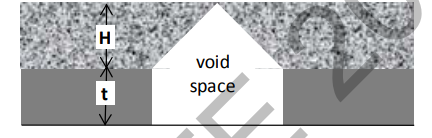
\includegraphics[width=0.4\columnwidth]{figs/flat coal.png}
  \caption{Opencast Mine}
  \label{fig:30}
\end{figure}


\hfill\brak{GATE\ MN\ 2014}

\item A piece of coal sample weighs $10$ kg in air and $2$ kg when immersed in water. The specific gravity
of the coal sample is

\hfill\brak{GATE\ MN\ 2014}

\item In a borehole log of $1.2$ m in length, recovery of rock cores in cm is given below
$20$, $8$, $15$, $8$, $8$, $4$, $3$, $9$, $10$, $1$, $5$, $10$ 
the RQD in percentage is 

\hfill\brak{GATE\ MN\ 2014}

\begin{multicols}{4}
\begin{enumerate}
\item $29.2$
\item $31.8$
\item $45.8$
\item $50.0$
\end{enumerate}
\end{multicols}

\item An underground coal mine panel produces $520$ tonnes per day deploying $220$, $200$ and $192$ persons
in three shifts. As per CMR $1957$, the minimum quantity of air in $m^3$/min to be delivered at the last ventilation connection of the panel is

\hfill\brak{GATE\ MN\ 2014}

\item In A PERT Network the activities on the critical path are a, b and c. The standard deviations of the durations of these activities are 2, 2 and 1 respectively. The variance of the project duration is 

\hfill\brak{GATE\ MN\ 2014}
\begin{multicols}{4}
\begin{enumerate}
\item $3$
\item $5$
\item $9$
\item $12$
\end{enumerate}
\end{multicols}

\item A particle $P$ is in equilibrium as shown in the figure. The magnitude in kN and the orientation $\theta$ in degrees of the force $\mathbf{F}$ respectively are 
\begin{figure}[H]
  \centering
  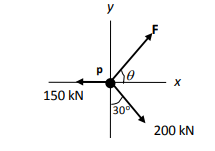
\includegraphics[width=0.4\columnwidth]{figs/diagram.png}
  \caption{diagram}
  \label{fig:36}
\end{figure}

\hfill\brak{GATE\ MN\ 2014}
\begin{multicols}{4}
\begin{enumerate}
\item $5952.1$,$16.1$
\item $221.2$, $23.2$
\item $ 102.3$, $53.4$
\item $180.3$, $73.9$
\end{enumerate}
\end{multicols}

\item A distributed load of $4$ kN/m acts on a beam of $6$m length supported by a hinge and a roller as shown in the figure. The distance in m of the point of zero shear in the beam from the point A is 
\begin{figure}[H]
  \centering
  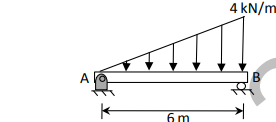
\includegraphics[width=0.4\columnwidth]{figs/load.png}
  \caption{Load}
  \label{load}
\end{figure}

\hfill\brak{GATE\ MN\ 2014}

\item A dry rock sample of diameter $50$ mm and length $100$ mm weighs $300$ g. After saturating in brine
solution of specific gravity $1.05$, its weight increased to $330$ g. The porosity of the rock sample in
percentage is

\hfill\brak{GATE\ MN\ 2014}

\item A joint plane of length $L$ and dip $\delta$ intersects the toe of a slope as shown in the figure. The weight of the shaded block is $W$. Uniform water pressure $P$ acts normal to the joint plane. If the cohesion and angle of internal friction of the joint surface are $c$ and $\phi$ respectively, then the expression for `safety factor' of the shaded block is 
\begin{figure}[H]
  \centering
  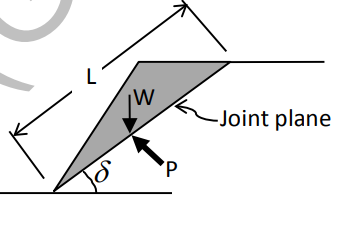
\includegraphics[width=0.4\columnwidth]{figs/dia2.png}
  \caption{dia}
  \label{daigram2}
\end{figure}

\hfill\brak{GATE\ MN\ 2014}
\begin{multicols}{2}
\begin{enumerate}
\item  $\dfrac{Lc + (W \sin \delta - LP)\tan \phi}{W \cos \delta}$ 
\item  $\dfrac{Lc + (W \cos \delta + LP)\tan \phi}{W \sin \delta}$
\item  $\dfrac{Lc + (W \cos \delta - LP)\tan \phi}{W \sin \delta}$
\item  $\dfrac{Lc + (W \sin \delta + LP)\tan \phi}{W \cos \delta}$
\end{enumerate}
\end{multicols}

\item The lengths and standard errors of three sections AB, BC, and CD of a straight line AD are given
below
$AB = 125.85 \pm 0.021 \,\text{m}; \; 
BC = 205.72 \pm 0.029 \,\text{m}; \; 
CD = 246.21 \pm 0.025 \,\text{m}$

\hfill\brak{GATE\ MN\ 2014}
\begin{multicols}{4}
\begin{enumerate}
\item $\pm 0.0436$
\item $\pm 0.0350$
\item $\pm 0.0250$
\item $\pm 0.0019$
\end{enumerate}
\end{multicols}

\item  The bearing of side $AB$ of a regular hexagon $ABCDEF$ is $S \, 50^{\circ}10' \, E$. If the station $C$ is easterly from the station $B$, the whole circle bearing of the side $BC$ is  

\hfill\brak{GATE\ MN\ 2014}
\begin{multicols}{4}
\begin{enumerate}
\item $65^{\circ}15'25''$
\item $69^{\circ}50'25''$ 
\item $69^{\circ}15'25''$
\item $69^{\circ}50'0''$
\end{enumerate}
\end{multicols}

\item  In a room-and-pillar stope, bench blasting is conducted using ANFO having density of $800 kg/m^3$The specific gravity of rock is $2.5$, hole diameter is $100$ mm and spacing to burden ratio is $1.3$.The
charge length of each blast hole is 80\% of the hole length. For a desired powder factor of 0.48 kg/tonne, the spacing and burden of the blast pattern in m respectively are

\hfill\brak{GATE\ MN\ 2014}
\begin{multicols}{4}
\begin{enumerate}
\item $-5$
\item $+5$
\item $-2$
\item $+2$
\end{enumerate}
\end{multicols}
\item Match the following for ore handling operations in an underground metal mine
\begin{table}[H]
  \centering
  \caption{Match The Following}
  \begin{tabular}{>{\bfseries}l l}
Specification & Outer Diameter in mm \\
P. AW & p. 34.9 \\
Q. BW & q. 44.4 \\
R. EW & r. 54.0 \\
S. NW & s. 66.7 \\
\end{tabular}


  \label{tab:table1}
\end{table}
\begin{multicols}{2}
\begin{enumerate}
\item P-IV, Q-III, R-II, S-I
\item P-III, Q-IV, R-I, S-II
\item P-II, Q-IV, R-I, S-III
\item P-III, Q-I, R-II, S-IV
\end{enumerate}
\end{multicols}

\item The following characteristic curves (P, Q, R, S) pertain to rotary drilling in rock. 
\begin{figure}[H]
  \centering
  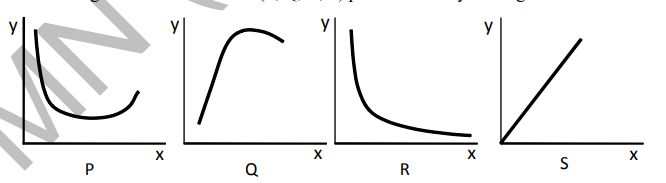
\includegraphics[width=0.4\columnwidth]{figs/Graph.png}
  \caption{graph}
  \label{fig:37}
\end{figure}
\begin{enumerate}
    \item Torque versus RPM
    \item Rate of penetration versus uniaxial compressive strength of rock
    \item Rate of penetration versus weight on bit
    \item Specific energy versus weight on bit
\end{enumerate}

\hfill\brak{GATE\ MN\ 2014}
\begin{enumerate}
\item P-III, Q-IV, R-II, S-I
\item P-II, Q-IV, R-I, S-III
\item P-IV, Q-III, R-II, S-I
\item P-I, Q-III, R-II, S-IV
\end{enumerate}

\item The height $H$ of a drawpoint in a sublevel caving stope is $3.0 \, \text{m}$. If the angle of repose $(\varphi)$ of broken ore is $35^{\circ}$, the digging depth $y$ of the loader as shown in the figure in m is \underline{\hspace{2cm}}.

\hfill\brak{GATE\ MN\ 2014}
\begin{figure}[H]
  \centering
  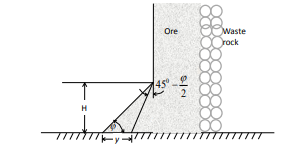
\includegraphics[width=0.4\columnwidth]{figs/wall.png}
  \caption{illustration}
  \label{fig:wall}
\end{figure}
\item The area enclosed by the curves $y = x^2$ and $y = x^3$ for $x \in [0,\infty)$ is

\hfill\brak{GATE\ MN\ 2014}
\begin{multicols}{4}
\begin{enumerate}
\item $1/12$
\item $1/6$
\item $1/2$
\item $1$
\end{enumerate}  
\end{multicols}
\item For an explosives company, the probability of producing a defective detonator is $0.02$. The
probability that a lot of $50$ detonators produced by the company contains at most $2$ defective
detonators is 
\hfill\brak{GATE\ MN\ 2014}
\item The area enclosed by the curves $y = x^{2}$ and $y = x^{3}$ for $x \in [0,\infty)$ is 

\hfill\brak{GATE\ MN\ 2014}

\begin{multicols}{4}
\begin{enumerate}
\item $\frac{1}{12}$
\item $\frac{1}{6}$
\item $\frac{1}{2}$
\item $1$
\end{enumerate}
\end{multicols}

\item The value of $a$, for which the function below is continuous at $x = 1$ is
\[
f(x) =
\begin{cases}
2x + ax^2, & x \leq 1 \\
4x + 3, & x > 1
\end{cases}
\]
\hfill\brak{GATE\ MN\ 2014}
\begin{multicols}{4}
\begin{enumerate}
\item $13.09$
\item $12.50$
\item $11.74$
\item $10.87$
\end{enumerate}
\end{multicols}

\item The sum of the infinite series 
$a + ar + ar^{2} + ar^{3} + \cdots + ar^{n-1} + \cdots \quad \text{for } |r| < 1$
is
\hfill\brak{GATE\ MN\ 2014}

\begin{multicols}{4}
\begin{enumerate}
\item $a(1+r)$
\item $a(1-r)$
\item $\frac{a}{1+r}$
\item $\frac{a}{1-r}$
\end{enumerate}
\end{multicols}

\item A centrifugal pump has a discharge rate of $2000$ L of water per min against a total head of $200$ m. If the pump efficiency is $75$\%, the input power to the pump in kW is

\hfill\brak{GATE\ MN\ 2014}
\begin{multicols}{4}
\begin{enumerate}
\item $87.20$
\item $49.05$
\item $ 13.33$
\item $7.50$
\end{enumerate}
\end{multicols}

\item  A dragline is required to remove $3,00,000$ $m^3$ of rock per month on the bank volume basis.
Consider the following data for the dragline operation.\\
Effective working hours per month = 450,
Bucket fill factor = $0.8$,
Cycle time = $65$ s,
Swell factor of the rock = $1.25$,
The minimum bucket capacity of the dragline in $m^3$ is

\hfill\brak{GATE\ MN\ 2014}
\begin{multicols}{4}
\begin{enumerate}
\item $7.70$
\item $9.63$
\item $12.04$
\item $ 18.80$
\end{enumerate}
\end{multicols}

\item A direct rope haulage pulls $8$ tubs loaded with coal through an incline of length $500$ m having an
inclination of $1$ in $6$. Consider the following additional data.
Capacity of tub = $1.0$ tonne
Tare weight of tub = $500$ kg
Hauling speed = $9$ km per hour
Coefficient of friction between wheel and rail = $1/60$
Coefficient of friction between rope and drum = $1/10$
Mass of rope per meter = $1.5$ kg 
The minimum power required to haul the tubs in kW is

\hfill\brak{GATE\ MN\ 2014}
\begin{multicols}{4}
\begin{enumerate}
\item $345.50$
\item $348.60$
\item $350.10$
\item $365.50$
\end{enumerate}
\end{multicols}

\item A coal mine receives two bids for purchase of a new dragline. The first bid quotes Rs. $150$ crore as a price to be paid in full on delivery. The second bid quotes Rs. 180 crore as a price payable at the end of the third year after delivery. If the discount rate is $12$\%, the difference in NPV between the first and second bids in crore of rupees is

\hfill\brak{GATE\ MN\ 2014}

\item Match the following in the context of underground mine environment:
\begin{table}[H]
  \centering
  \caption{Match The Following}
  \begin{center}
\begin{tabular}{|c|c|c|c|c|c|}
\hline
Mass of particles, g      & 2   & 5   & 7   & 4   & 1    \\
\hline
Mean size of particles, $\mu$m & 350 & 240 & 200 & 150 & 100 \\
\hline
\end{tabular}
\end{center}
  \label{tab:Table1}
\end{table}

\hfill\brak{GATE\ MN\ 2014}
\begin{multicols}{2}
\begin{enumerate}
\item P-II, Q-I, R-III, S-IV
\item P-III, Q-IV, R-I, S-II
\item P-IV, Q-II, R-III, S-I
\item P-I, Q-III, R-IV, S-II
\end{enumerate}
\end{multicols}

\item  A mine airway having cross-section of $2.2 \,\text{m} \times 2.2 \,\text{m}$ 
and length $500 \,\text{m}$ contains a bend. 
Given that the airway friction factor is $0.01 \,\text{Ns}^2\!/\text{m}^4$, 
shock loss factor for the bend is $0.07$, 
and density of air is $1.2 \,\text{kg}/\text{m}^3$, 
the equivalent length of the airway in m is

\hfill\brak{GATE\ MN\ 2014}
\item  In order to estimate the NVP in a mine,measurements are made at the main fan as shown below.
\begin{table}[H]
  \centering
  \caption{Match The Following}
  \begin{table}[ht]
\centering
\begin{tabular}{|l|l|}
\hline
\textbf{Column I} & \textbf{Column II} \\ \hline
P. Hydraulic Conductivity   & 1. Upper limit of moisture available to plant \\ \hline
Q. Permeability            & 2. All soil pores are filled with water         \\ \hline
R. Viscosity               & 3. Soil capillarity                            \\ \hline
S. Surface Tension         & 4. Properties of fluid as well as soil          \\ \hline
T. Saturation Capacity     & 5. Property of the medium                      \\ \hline
U. Field Capacity          & 6. Internal friction that brings about resistance to flow \\ \hline
\end{tabular}
\end{table}
  \label{tab:Table3}
\end{table}

\hfill\brak{GATE\ MN\ 2014}
\item The NVP is $\colon$
The resistances of two splits A and B are 
$0.35 \,\text{Ns}^2\text{m}^{-8}$ and 
$0.05 \,\text{Ns}^2\text{m}^{-8}$ respectively. 
The combined resistance of the shafts and trunk airways is 
$0.4 \,\text{Ns}^2\text{m}^{-8}$. 
A booster fan is planned to be installed in split A to increase the quantity flowing through it. 
Assuming that the surface fan continues to operate at a constant pressure of $1000 \,\text{Pa}$, 
the critical pressure of the booster fan in Pa is $\colon$

\hfill\brak{GATE\ MN\ 2014}
\item A pitot tube is inserted in a ventilation duct with the nose facing the air flow. A vertical U-tube
manometer filled with alcohol (specific gravity $0.8$) has been used for pressure measurements such that $10.2$ mm is read as the total pressure and 8.8 mm as the static pressure. Given the density of air to be $1.2$ $kg/m^3$
, the air velocity at the nose of the pitot tube in $m/s$ is $\colon$

\hfill\brak{GATE\ MN\ 2014}
\begin{figure}[H]
  \centering
  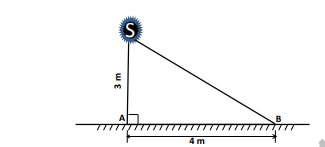
\includegraphics[width=0.4\columnwidth]{figs/figtri.png}
  \caption{Illustration for Q49}
  \label{fig:tri}
\end{figure}
\item An illumination source S shown in the figure emits light equally in all directions. At a point A on
the floor, the illuminance is $5.0$ lux. The illuminance at point B on the floor in lux is

\hfill\brak{GATE\ MN\ 2014}
\item Two machines A and B while operating simultaneously produce a sound pressure level of $85$ dBA at a point. When the machine A stops, the sound pressure level at that point reduces to $80$ dBA. The sound pressure level at the same point due to machine A operating alone in dBA is


\hfill\brak{GATE\ MN\ 2014}
\begin{multicols}{4}
\begin{enumerate}
\item $70.0$
\item $75.0$
\item $80.0$
\item $83.3$
\end{enumerate}
\end{multicols}
\item A waste water effluent has BOD5 of $80$ mg/L and the reaction rate constant is $0.16$ per day. The ultimate BOD in mg/L is
\hfill\brak{GATE\ MN\ 2014}
\begin{multicols}{4}
\begin{enumerate}
\item $85$
\item $100$
\item $120$
\item $145$
\end{enumerate}
\end{multicols}


\item A series of tri-axial compression tests conducted on sandstone samples reveal the following relationship between major and minor principal stresses:
\[
\sigma_{1} = 50 + 3\sigma_{3} \quad \text{[stresses are in MPa]}
\]

The cohesion in MPa and angle of internal friction in degrees of sandstone respectively are $\colon$


\hfill\brak{GATE\ MN\ 2014}

\begin{multicols}{4}
\begin{enumerate}
\item $14.43, \; 30.0$
\item $14.43, \; 60.0$
\item $0.21, \; 73.9$
\item $0.21, \; 16.1$
\end{enumerate}
\end{multicols}

\item Six detonators each having resistance of $1.5$ ohm are connected in parallel. A $15$ V exploder is connected to the detonators by two single-core cables of resistance $3$ ohm each. The current in the circuit in Ampere is $\colon$

\hfill\brak{GATE\ MN\ 2014}
\item  The failure and repair rates of a shovel are 
$0.06 \,\text{hr}^{-1}$ and $0.04 \,\text{hr}^{-1}$ respectively. 
\begin{figure}[H]
  \centering
  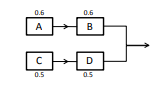
\includegraphics[width=0.4\columnwidth]{figs/flow.png}
  \caption{Flowchart}
  \label{fi}
\end{figure}
The individual reliability values of four sub-systems are given in the figure below. The reliability of
the system is
\begin{center}
\Large\textbf{{END OF THE QUESTION PAPER}}
\end{center}
\end{enumerate}
\end{document}